\chapter{Alignment with Tandem Repeats} \label{CHAPTER:REP}
\firstUseOf{Tandem repeat} is a region in the genomic sequence that contain two
or more consecutive repetitions of some \firstUseOf{motif}, which is a short
genomic sequence. Instances of motif in tandem repeat are called
\firstUseOf{repetitions}.  Tandem repeats, like other sequences, undergo
evolution and therefore events like mutations, insertions, and deletions
occurs in the individual repetitions.  Therefore individual repetitions are only an approximate copies of a motif.
More than $2\%$ of the human genome is covered by short
tandem repeats, and they occurs in many genes and regulatory regions
\cite{Gemayel2010}. Additionally, recent short insertions in human genome are
mostly caused by tandem duplication \cite{Messer2007}. Most of the tandem
repeats evolved using tandem segmental duplications, which means that tandem
repeat was created using several duplication events. The consequence is that
the homologous tandem repeats in two related sequences can contain variable
number of copies of the original motif. Note that it is highly likely that none
of the repetition is exact copy of original motif.

Aligning homologous tandem repeats is hard, because it is not clear which
copies of tandem repeat are orthologous (created by speciation, not duplication
within same genome) and which are paralogous (created by duplication event in
only one sequence). Tandem repeats does not only affect quality of alignment
within them, but error spread into adjacent columns of an alignment as we show
in Section \ref{SECTION:REPSIMRESULTS}, Figure \ref{FIGURE:SFF_GRAPHS}.  These
inaccuracies can spread further and cause artifacts in the results of
comparative genomic methods that uses sequence alignments.

In this chapter we introduce tractable model that explicitly accounts for
tandem repeats. We use the maximum expected gain framework to explore several
decoding criteria for our model. We evaluate our model using simulated data. 

\section{Methods for Aligning Tandem Repeats}\label{SECTION:REPALNMETHODS}

Alignment with tandem duplications were first studied by Benson
\cite{Benson1997}, who proposed extension of the Needleman-Wunsch algorithm. In
their scoring scheme, they scored duplications as an separate event. Each
duplication was penalized by the duplication initiation cost, the duplication extension
costs for each copy and Needleman-Wunsch like scoring scheme to score original
string with its repetitions. Time complexity of his algorithm was $O(n^4)$ and
Benson proposed heuristic algorithm to compute alignment in reasonable time.
Additional work was done by alternative incorporation of tandem duplication
(and other operations) into the scoring schemes \cite{Sammeth2006, Berard2006,
Freschi2012}, or using lossy compression scheme that collapsed tandem repeats,
then aligned compressed sequences \cite{Freschi2012}.

Traditional approach to deal with tandem repeats is to mask tandem repeats in
both sequences and then aligned masked sequences by some alignment algorithm.
Masking is replacing low complexity regions (e.g. tandem repeats) either with
lower-case letters (soft-masking) or with N symbols (hard-masking, N represents
any base). Masking is done by method for finding tandem repeats, such as
\abbreviation{Tandem Repeat Finder}{TRF} \cite{Benson1999}, TANTAN
\cite{Frith2011}, mreps \cite{Kolpakov2003}, or ATRhunter \cite{Wexler2005}. 

Methods mentioned above were not probabilistic methods. The first probabilistic
method specifically targeting tandem repeats was introduced by Hickey and
Blanchette \cite{Hickey2011}.  They developed context-sensitive model based on
pair Tree-Adjoining grammars.  Their model does not explicitly model arbitrary
number of copies of repetitive region, it focused on short context sensitive
indels caused by tandem duplications, because majority ($90\%$
\cite{Hickey2011}) of short indels are caused by tandem duplication. Time
complexity for their decoding algorithm was $O(n^2L^2)$, where $n$ is the
length of the sequences and $L$ is the maximal length of context sensitive
indels.

Another, not entirely probabilistic method was developed by Kováč {\it et. al
(2012)}\nocite{Kovac2012}. Aim of the method was to align repetitive motif
inside some protein families (for example zinc finger proteins), which are
similar to the tandem repeats. Their method focused on correctly aligning
individual occurrences of the motifs. They combined profile HMM and pair HMM,
and developed new decoding algorithm similar to the Viterbi algorithm. Despite
usage of probabilistic models, their method was not a probabilistic model. 

Hudek \cite{Hudek2010} developed algorithm that is mixture of the Viterbi and
posterior decoding. The goal of the algorithm was to reduce the misalignments
due to short tandem repeats with the consensus length $1$, for example $AA$
in the first sequence and $AAAAAAAAA$ in the second sequence. Algorithm
developed by Hudek was considering all possible alignments of $u$ and $v$ in
the final alignment. Algorithms goal was to segment alignment into blocks, such
that each block contain gaps only in one sequence. They developed pHMM model
that defines probability distribution over all possible segmentation of
alignments of input sequences and give the algorithm that finds the most
probable segmentation.  Unlike Viterbi algorithm, their algorithm considers all
possible alignments within each segment.

\section{Models and Methods Searching Tandem Repeats}

In this section we describe methods and models we used for improving
performance of our methods or as a parts of larger model for aligning sequences
with tandem repeats. 

\subsection{Tandem Repeat Finder}

Probably the most popular method for searching for tandem repeats is to use TRF
\cite{Benson1999}.  Tandem repeat finder find the position of tandem repeats
(referred as an \firstUseOf{interval}), consensus sequence (the approximation
of original motif), alignment of the consensus sequence and the input sequence,
and various other information about repeats.

Method consists from two components: detection and analysis. Detection
component tries to find a set of candidate tandem repeats by analyzing the
differences in the positions of matching $k$-tuples (subsequence of the input
sequence of length $k$). It uses several statistical criteria to detect repeats
and distinguish between tandem repeats and non-tandem repeats
\cite{Benson1999}.

Analysis component aligns candidate consensus using wraparound dynamic
programming \cite{Myers1989} with the surrounding sequence. If the alignment is
not successful (candidate consensus has to be aligned at least $2$ times to be
successful), candidate repeat is discarded. Otherwise, the final consensus
sequence is computed from the alignment along with other statistics about
tandem repeat.

Tandem repeats found by TRF can be redundant.  They can overlap, have slightly
different consensuses, the consensuses can be shifted cyclically, and can have
different lengths, as in following example:

\begin{verbatim}
Sequence  X:        CACCGCCACCACCGTAG
Consensus ACCACC:    ACCACCACCACC      2 repetitions
Consensus AAC:       ACCACCACCACC      4 repetitions
consensus CAC:      CACCACCACCACC      4.3 repetitions
\end{verbatim}

The sequence $X$ contain tandem repeat and there are three possible consensus
sequences with different number of repetitions. Note that the repetition of the
consensus can be incomplete; as with the $CAC$ consensus where we have $4.3$
($0.3$ stands for the last $C$ in the repetitive sequence). This is important
to know, because we will use the TRF to find the set candidate tandem repeats
of input sequences, not as the definitive list of repetitive regions.

Note that the purpose of this example to illustrate redundancy of TRF output.
If we ran TRF on sequence $X$, the output would be only repeat with $CAC$ as an
consensus.

\subsection{Sunflower Model}\label{SECTION:SUNFLOWERMODEL}
\firstUseOf{Sunflower model} is HMM that models tandem repeat of one
previously specified motif $C=c_0\dots c_{k-1}$. We developed it as a part of
our model for aligning sequences with tandem repeats in
section\ref{SECTION:REPMODELS}, but it can be also used as an simple tool for
searching for tandem repeats and we used it to improve the candidate set
(described in Section \ref{SECTION:REPOPT}) of tandem repeats from the TRF
program.

Sunflower is an extension of the profile HMM described in Section \ref{HERD:METHODS}
in Figure \ref{FIGURE:PROFILEHMM} (page \pageref{FIGURE:PROFILEHMM}). Sunflower
model is a circular version of the profile HMM where match states represent the
motif $C$. This model assumes that repetitions evolved from motif $C$
independently of each other. One can think about it as that at single point of
time, motif $C$ was copied several times forming tandem repeat, which then
undergo through simple evolution events: substitutions, deletions and
insertions. This does not accurately reflect the evolution history of tandem
repeat, but trying to model such evolution would lead to much more complicated
model.

\begin{figure}
\begin{center}
\begin{subfigure}[b]{0.5\textwidth}
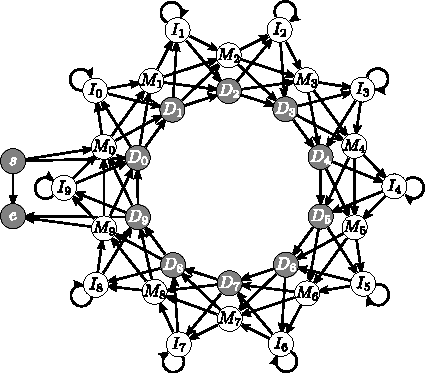
\includegraphics{../figures/SunflowerSilentCircle.pdf}
\caption{Cyclic profile model}\label{SUBFIGURE:SUNFLOWERSILENTCYCLE}
\end{subfigure}%
\begin{subfigure}[b]{0.5\textwidth}
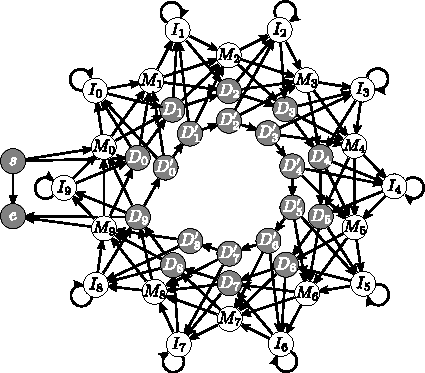
\includegraphics{../figures/Sunflower.pdf}
\caption{Sunflower model}\label{SUBFIGURE:SUNFLOWER}
\end{subfigure}
\end{center}
\caption[Example of the Sunflower model]{Example of the Sunflower model 
with the motif of length $10$. White states emit one character and gray states are
silent states. States $s$ and $e$ are initial and final silent states. Sunflower model
has additional delete states $D'_0, \dots D'_8$ to remove silent cycle from the
model.}
\label{FIGURE:SUNFLOWERMODEL}
\end{figure}

To model this process, we start with the profile HMM with motif $C$ and
circularize it: It contains states $M_0,\dots, M_{k-1}, I_{0}, \dots, I_{k-1}$
and $D_{0}, \dots, D_{k-1}$. The transitions between the states are similar to
profile HMM:  $M_{i}\to M_{i\oplus 1}, M_i\to I_i, M_i\to D_{i\oplus 1}, I_i\to
I_i, I_i\to M_{i\oplus 1}, I_i\to D_{i\oplus 1}, D_{i}\to D_{i \oplus 1},
D_{i}\to M_{i\oplus 1}, D_{i}\to I_i$ for all $0\leq i < k$, where $\oplus$ is
$+$ modulo $k$ (as opposed to the profile HMM). As in the profile HMM, $D_i$ states
are silent. Additionally we add silent start state $s$ and silent final state
$e$ with transitions $s\to M_0, s\to D_0, D_{k-1}\to e, M_{k-1}\to e$ and
transition $s\to e$ to model empty tandem repeat.  Whole model topology is in
Figure \ref{SUBFIGURE:SUNFLOWERSILENTCYCLE}.

The problem is that the cyclic profile contains cycle of silent states, which
causes problems with training and decoding algorithm, which was mentioned in
Section \ref{SECTION:SILENT}. Removing these states would lead to additional
$\theta(k^2)$ edges, or we would have to sacrifice the ability to delete arbitrary
(in cyclic sense) parts of motif. Therefore we have decided to remove
transition between delete states $D_{k-1}$ and $D_0$. To compensate to the lost
possibility of deleting arbitrary part of tandem repeat, we add additional
chain of delete states $D'_0, \dots, D'_{k-2}$ that are accessible only from
state $D_{k-1}$ by transition $D_{k-1}\to D'_0$, and their outgoing transitions
are similar to delete state transitions: $D'_{i}\to M_{i+1}, D'_{i}\to I_i$ for
$0\leq i\leq k-2$ and $D'_{i} \to D'_{i+1}$ for $0\leq i < k-2$. The full model
is in Figure \ref{SUBFIGURE:SUNFLOWER}. We call this model the
\firstUseOf{Sunflower} model.

This model has $4k+1$ states and $12k+1$ transitions, out of which $2k+1$
states are silent.  Since alphabet size is $4$, there are $14k+2$ parameters to
train for a motif $C$ (including emissions of insert and match states). Models
with such a large number of parameters are hard to train, so we reduced the
number of parameters. We tied similar transitions, so that they have the same
probability.  We ended with the set of parameters $p_{ab}$ where $a,b\in \{m,
i, d, \cdot\}$, where $m$ stands for any match state, $i$ stands for any insert
state, $d$ states for any delete state (from both chains), and $\cdot$ is
either start or final state. Therefore the probability of transition from match
state to delete state is $p_{md}$ and probability of transition from insert
state to final state is $p_{i\cdot}$.  Probabilities were set in a way, that
$\sum_{b\in\{m,i,d\} p_{ab}}=1$ for all possible $a$.  Therefore, transitions
from states $M_{k-1}, D_{k-1}$ and $D'_{k-1}$ does not sum to $1$, because they
are either missing one transition or having one additional transition. For
those states the probability of transitions were normalized in order to form a
probability distribution. 

Emission parameters were reduced in following way: all insert states share
the same emission distribution. For the emission distribution of match state $M_i$ we
assumed that base $c_i$ from the motif evolved over evolutionary time $t$
according to Jukes-Cantor model. Jukes-Cantor model is a theoretical model of evolution
that assumes constant rate of evolution. Under this model base $B_1$ evolved
over time $t$ to different base $B_2$  with probability $1/4(1-\exp(-4t/3))$.
The probability that $B_1$ after time $t$ will be still (or again) $B_1$  is
$1/4(1+3\exp(-4t/3))$ \cite{Durbin1998}. Time $t$ was same for all match
states. Therefore emissions of all states has only $4$ parameters ($1$ for
match states and $3$ for insert states).

\begin{note}
In Jukes-Cantor model, the parameter $t$ is not time as measured by
seconds/years. It is a branch length in evolutionary tree and it is
multiplication of substitution rate and time. We used this small inaccuracy to
simplify explanation.  More details can be found in \cite{Durbin1998}.
\end{note}

Sunflower model models only tandem repeats and it is not directly usable for
finding tandem repeats. To do so, it is necessary to add state $B$ that models
non-repetitive part of the sequence. Let $S_C$ be the Sunflower for motif  $C$.
We add the transitions from $B$ to the start state of $S_C$ and from the final
state of $S_C$ to the state $B$. The probability of transition from the state
$B$ to the submodel $S_C$ is $p_r$, the probability of repeat starting at
particular position in the sequence. Probability of transition from final state
of $S_C$ to $B$ is $1$.  There is also transition $B\to B$ with probability
$1-p_r$. We used the Viterbi algorithm with this model to find all occurrences
of tandem repeat with motif $C$. However, with this model we can search only
for specific motif. We call this method of finding tandem repeats the
\abbreviation{Sunflower repeat finder}{SRF}.

\subsection{TANTAN}\label{SECTION:TANTAN}

\firstUseOf{TANTAN} is a high-order HMM aimed for finding tandem repeat developed
by Frith \cite{Frith2011}. Unlike Sunflower model, TANTAN models tandem repeats
with an arbitrary motif. Its only restriction is the maximal length of the motif
$K$. In this section we describe the core of the model; the part that models
tandem repeats. This core can be transformed to the model usable for search by
same method as we described for Sunflower model.

\begin{figure}
\begin{center}
\begin{subfigure}{0.19\textwidth}
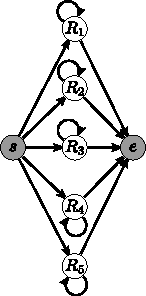
\includegraphics{../figures/tantan_simple.pdf}
\caption{Simple model}\label{FIGURE:TANTAN:SIMPLE}
\end{subfigure}%
\begin{subfigure}{0.3\textwidth}
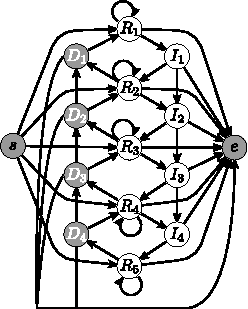
\includegraphics{../figures/tantan_indel.pdf}
\caption{With indels}\label{FIGURE:TANTAN:INDEL}
\end{subfigure}%
\begin{subfigure}{0.35\textwidth}
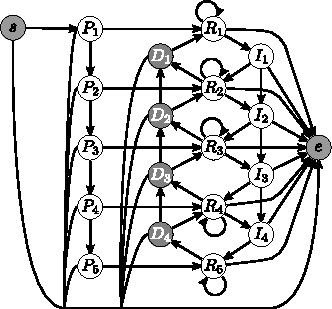
\includegraphics{../figures/tantan_init.pdf}
\caption{With first repetition}\label{FIGURE:TANTAN:INIT}
\end{subfigure}%
\end{center}
\caption{Three variants of the core of the TANTAN model. Gray states are
silent. The first one is simplified model, only with repeat states. The second
was used by Frith \cite{Frith2011}, allowing insertions and deletions.  The last one
is our extension with additional prefix states $P_1, \dots P_5$ that models
the first repetition.}\label{FIGURE:TANTAN}
\end{figure}

The principal idea is to use the state of order $l$ to model a repeat with
motif length $l$. TANTANs high order states uses less information than standard
high order states.  Standard high order state of order $l$ depends on
subsequence $X[i-l:i]$ where $X[i]$ is the symbol that is being emitted.
TANTANs states of order $l$ depends only on the symbol $X[i-l]$. Model consists
from $K$ high-order states $R_l$, $1\leq l\leq K$ called repeat states, where
state $R_l$ is of order $l$. Emission of state $R_l$ is set in such a way, that
state emits the same symbol as $X[i-l]$ with high probability. By adding
transition $R_l\to R_l$ we obtain HMM modeling tandem repeats without indels
with motif length $l$. By connecting states $R_1,\dots, R_K$ to single start
and final state as shown in Figure \ref{FIGURE:TANTAN:SIMPLE}, we obtain HMM
that models repeats with the motif lengths $1$ through $K$.

This simplified model does not allow insertions and deletions in the
repetition.  Idels are handled similarly to the profile HMMs, by adding insert
states $I_1,\dots, I_{K-1}$ and silent delete states $D_1, \dots, D_{K-1}$
connected as in the Figure \ref{FIGURE:TANTAN:INDEL}. There are however
significant difference from the profile HMM.  In profile HMM, delete states
were used to skip at least one match state, while in TANTAN delete state is
used move to state with lower order. Additionally, insert states moves in
opposite direction, using insert state causes increase of the order of the
repeat state.  It is also possible to move from the insert state $I_{j}$ to the
insert state $I_{j+1}$ which is not possible in the profile HMM.

One disadvantage of the TANTAN model is that it does not model the first
occurrence of the motif sequence, since repeat states model only the
repetitions of the sequence. This caused problems when we wanted to incorporate
TANTAN as a submodel for aligning sequences. Therefore we have added additional
chain of prefix states $P_1,\dots, P_K$ modeling the first repetition. Transitions
from the start state are now only to the final state (modeling empty sequence) and
the state $P_1$. State $P_l, 1\leq l\leq K$ has transitions to the final state,
repeat state $R_l$ and the state $P_{l+1}$, if such state exists.

%Emisie a sme hotovy
We set emission distribution of the insert and prefix states to the background
probability: the distribution of the bases in DNA. Emission state of the state
$R_l$ was derived using Jukes-Cantor model with parameter $t$, where the
emission $X[i]$ evolved from $X[i-l]$ over time $t$.

\section{Models for Aligning with Tandem Repeats}\label{SECTION:REPMODELS} In
this section we describe models that we have used in our methods. We describe
model in an dual way; as an generalized pHMM and as an equivalent
non-generalized pHMM (emissions length are at most $1$ in both sequences). By
equivalency we mean that the distribution of generated alignments and
annotations (with certain annotation function) are same, but clearly the
distribution of state paths will be different due to different sets of states.

Generalized model is obtained by taking simple 3-state pHMM model from section
\ref{SECTION:ALIGNWITHPHMM} and adding single generalized pair state $R$,
called the \firstUseOf{repeat state}, which in a single step generates tandem
repeats in both sequences. The state $R$ can in theory generate arbitrary long
sequences and it does not produce an alignment of tandem repeats during
decoding. Its task is to filter out tandem repeats of alignment, so that they
do not cause biases in the parts of an alignment emitted by other states (match
and indel states). We align homologous tandem repeats later in the
post-processing step. The overall topology of GpHMM is illustrated in the
Figure \ref{FIGURE:REPEAT_GENERAL}.

To made this model more flexible, the emission distribution of the state $R$ is
defined by an additional pHMM. Since the repetitions in the tandem repeat are
very similar to each other, we did not try to model the evolution of repetitive
parts of the sequences. We assumed that repeats generated by one emission of
the state $R$ from single motif and then evolved independently. Model was
constructed from the Sunflower models. Let $C$ be the set of all motifs that
can occur in the alignment. For each motif $c\in C$ we created sunflowers
$S_c^X$ and $S_c^Y$.  Sunflower $S_c^X$ is pairwise sunflower model with motif
$c$ that generates symbols only in sequence $X$, $S_c^Y$ is analogous.  We
connect $S_c^Y$ and $S_c^X$ by transition from the final state of $S_c^X$ to
the start state of $S_c^Y$ with probability $1$ and thus getting model $H_c$
that generates repeats in both sequences. We connected models $H_c$ for $c\in
C$ in parallel by single start and single end state as in the Figure
\ref{FIGURE:REPEAT_GENERAL}. The probability of the transition from the start
state to the start state of model $H_c$ was determined from the distribution of
motifs $\prob{c}$. Note that the size of this model is determined mostly by the
total length of all motifs and therefore this model can be very large, even
infinite if we consider all possible sequences as an possible motif for a
tandem repeat.  To keep the model size small, we computed a set of candidate
motifs $C$ and use it for construction of model. More details are in the
section \ref{SECTION:REPOPT}. We call this generalized model the
\abbreviation{sunflower field}{SFF} model.

\begin{figure}
\begin{center}
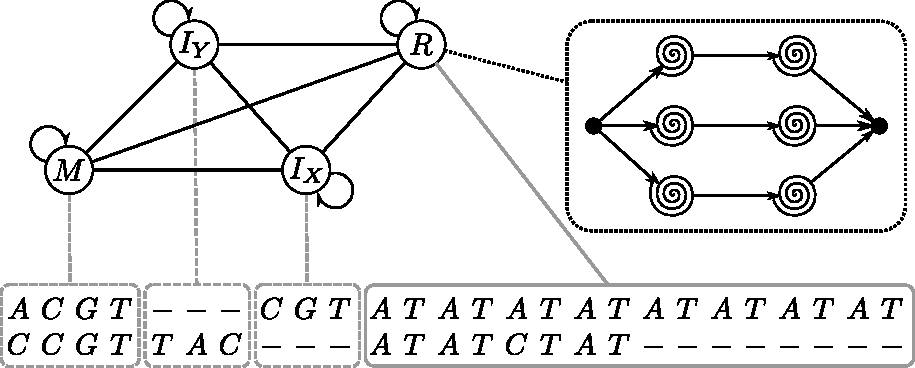
\includegraphics[width=14cm]{../figures/PairRepeatHMMGeneral.pdf}
\end{center}
\caption[General topology of Repeat pHMM]{ 
Topology of Repeat pHMM. We extended 3-state pHMM with one generalized states
$R$, that in one emission generates tandem repeats in both sequences. The
emission distribution of $R$ state is defined by another pHMM. Gray lines
represents emissions: dashed lines corresponds to multiple emissions from same
states, while full line represents one emission. Dotted black line represents
connection to submodel that is used for generating tandem repeats.

Black states in submodel on the right are silent start and end states. Spirals
represents submodels generating tandem repeat in one sequence. They are in
pairs of two identical models, one for generating tandem repeat in one
sequence, other for generating tandem repeat in other sequence. There are
multiple pairs of submodels, each for modeling different motif.
 }\label{FIGURE:REPEAT_GENERAL} 
\end{figure}

We also experimented with using TANTAN-like model for defining emissions
distribution of the state $R$. We used TANTAN model with the prefix states from
Section \ref{SECTION:TANTAN}. Similarly as with the sunflower model, we created two
copies of TANTAN, each generating repeats in only one sequence and connect them
together exactly as we would connect the sunflower models. Since TANTAN model does
not rely on a motif, it is not necessary to create more copies of TANTAN HMM and
its general topology looks like SFF's with only one motif.  Since TANTAN is
a high order HMM, resulting model is high order and generalized pair HMM. We
refer to this model as \abbreviation{TANTAN pHMM}{TTP}. Advantage of this model
over SFF is in it's size, since TTP will have in practice less states than SFF.
However, TTP models evolution of repetitions differently, since each repetition
is created from previous repetition and tandem repeats in sequences $X$ and $Y$
are independent of each other; there is no penalty for having different motifs.

SFF and TTP are defined as an $4$ state hight order GpHMM.  In general, using
generalized models increase the time complexity of decoding algorithms
quadratically. Therefore we also used expanded versions of the models: we
replaced generalized state $R$ with model defining emissions of $R$ (referred
as a submodel). All transitions entering into $R$ were replaced with the
transition to the start state of the submodel, and all outgoing transitions
from $R$ were replaced by transitions starting in final state of the submodel.
Distributions of alignments generated by this pHMM has not changed.
Additionally, the distribution of an annotation of an alignment did not
changed, if we use following annotation functions: For original GpHMM we use
identity function as a labeling function $\Lambda_{ID}$. For expanded model we
use function $\Lambda_R$, which label all states from submodel by label $R$,
and labels for other states is same as for GpHMM. 

\paragraph{Parameter estimation:}
We used $310,091$ consensuses found by the TRF program on the human chromozome
15 and its orthologous sequences in the dog genome as motifs for building SFF.
The probability of choosing particular motif was the observed frequency of the
motif in the TRF output. In practice, we limit the Sunflower submodels only to
those which was found by the TRF in the input sequence.  Additionally, if the
input sequence contain motif that is not in the predefined set, we add it to
the model with the probability of the least occurring motif in the model.

We set the parameters of the Sunflower submodel manually: the insert and delete
rates were set to $0.005$, the match states allows mutations from motif
sequence according to the Jukes-Cantor model with parameter $t=0.05$. The
emission of the insert states were set according to the frequency of the bases
in the input human-dog alignment.  Parameters of the TANTAN submodel were
estimated by the Baum-Welch algorithm \cite{Durbin1998} on 500 repeats sampled
from SFF.

The size of the TTP model depends on the length of the longest possible motif,
which we to to the $50$ bases. The size of the SFF model depends of the total
length of all motifs used. Therefore SFF can be exponentially larger than TTP
model. SFF model models assumes that repetitions were developed independently,
while the TTP model assumes that repetition evolves from the previous
occurrence of the repetition. Additionally, there is no dependence of tandem
repeats between sequence for TTP model.

Tandem repeats at orthologous positions in two species may share common
ancestor and therefore share part of their evolutionary history. However, it is
possible that they were consequently modified by additional evolution events
after speciation (including more tandem duplications). In our model we ignore
such a complex evolution of repetitions, because it would lead to very complex
model and increase the difficulty in decoding and training. Kováč {\it et. al}
developed method with limited dependence by adding repeat submodels emitting
copies in the two sequences at same time \cite{Kovac2012}.

\section{Decoding methods}\label{SECTION:REPDECODING}
In this section we describe several optimization criteria that we used with
3-state model, SFF model and TTP model: the \abbreviation{Viterbi
algorithm}{VA}, the \abbreviation{posterior decoding}{PD}, the
\abbreviation{marginalized posterior decoding}{MPD}, the \abbreviation{block
Viterbi algorithm}{BVA} and the \abbreviation{block posterior decoding}{BPD}.
The first three methods are used with the non-generalized models, the latter
two methods (block methods) are used with generalized version of the model. We
have already described first three algorithms in Section
\ref{SECTION:ALNDECODING}.  We introduce the highest expected gain framework
for pair HMM and formulate all algorithms using gain functions.

In Section \ref{SECTION:HEG} we defined gain functions as the functions of two
annotation. For pair HMMs we define gain function as an function of annotated
alignment: alignment columns along with annotation symbols. This is necessary
because we use generalized models, and therefore annotation symbols does not
uniquely determine alignment (there can be multiple alignments with the same
annotation).

We represent an annotated alignments using indices to
sequences and annotation symbols. In the case of generalized models, which can
generate more than one column, only the first column will contain state, other
columns will contain symbol $\varnothing$. Formally, \firstUseOf{annotated
alignment} of length $t$ of sequences $X=x_0x_1\dots x_{n-1}$ and
$Y=y_0y_2\dots y_{m-1}$ is represented as sequence of tuples $(u_0, a_0, b_0),
\dots, (u_{t-1}, a_{t-1}, b_{t-1})$ where $a_i\in \{0, \dots, {n-1}\}\cup\{-_0,
\dots, -_n\}$ and $b_i \in \{0, \dots, m-1\}\cup\{-_0, \dots, -_m\}$, and $u_i$
is either annotation symbol or symbol $\varnothing$. Number $i$ represents
$i$-th symbol in corresponding input sequence and $-_i$ represents gap in the
sequence before position $i$ (if $i$ is the length of the sequence, it
represents the gap at the end of the sequence). For example $(I_X, 47, -_{42})$
means that $x_{47}$ is aligned to a gap that is between $y_{41}$ and $y_{42}$
and that this column has annotation $I_X$. Naturally, indices in $a_i$ and
$b_i$ have to be non-decreasing order, each non-dashed symbol have to be in the
corresponding sequence in alignment exactly once. Additionally, $a_0$ has to be
$0$ or $-_{0}$, $a_t$ is $n$ or $-_m$. The constrains for $b$ are analogous.
The first annotation symbol $u_0\not=\varnothing$ and if some $u_i$ is equal to
$\varnothing$ then such column was emitted by same emission as previous column.
If we use non-generalized model, the annotated alignment cannot contain symbol
$\varnothing$. The reason for using annotation symbol $\varnothing$ is that we
will need to be able to distinguish between different generalized emissions. We
can define the probability of an annotated alignment $\Lambda$ as the sum of
the probabilities of the state paths that generate such an alignment and the
state paths annotation is equal to the annotation from $\Lambda$. We denote
this probability as $\prob{\Lambda\mid X, Y}$. We will refer to triple $(u_i,
a_i, v_i)$ as an \firstUseOf{annotated alignment column}.

We are interested in the \firstUseOf{repeat annotation} with annotation
function $\lambda_R$.  For generalized SFF and TTP (and 3-state pHMM),
$\lambda_R$ is identify function. For non-generalized version, $\lambda_R(u)=R$
for all states $u$ from submodel modeling tandem repeats.  The probability of a
state path and annotation is defined exactly as for HMM that generates only one
sequence.

Similarly as with the regular HMMs, we can define gain functions for annotation
alignment $G(\Lambda, \Lambda')$ that corresponds to ``similarity'' of two
annotated alignments (Note that for HMMs, symbol $\Lambda$ represents
annotation. With pHMM, we use this symbol for an annotated alignment).  Since pHMM
define the probability distribution $\Lambda_T$ of the correct annotated
alignments, we can define the expected gain of an annotated alignment given
sequence $X$ and $Y$ and gain function $G$: 
\begin{equation}
E_{\Lambda_T\mid X, Y}\left[G(\Lambda_T, \Lambda)\right] = 
\sum_{\Lambda_T}G(\Lambda_T, \Lambda)\prob{\Lambda_T\mid X, Y}
\end{equation}

Since we do not know the correct annotated alignment, we search for the
annotated alignment $\Lambda^*$ with the highest expected gain:

\begin{equation}
\Lambda^* = \arg\max_{\Lambda}
E_{\Lambda_T\mid X, Y}\left[G(\Lambda_T, \Lambda)\right]
\end{equation}

Finally, we express optimization criteria of various decoding methods using
highest expected gain framework.

\paragraph{The Viterbi algorithm and block Viterbi algorithm} Gain function for
the Viterbi algorithm assigns $+1$ if the predicted annotated alignment is identical to true
annotated alignment. Optimization algorithm for non-generalized model was
described in the section \ref{SECTION:PAIRHMMVITERBI}. The time complexity is
$O(nmE)$ where $E$ is the number of non-zero transitions in the model. We will
discuss the time complexity for the generalized model in the end of this
section.

We make distinction between the VA and BVA when using SFF or TTP models. Using
the VA on the expanded model is referred to as the VA. Using the VA on the
generalized version of the model will be referred as the BVA. The difference
between these two versions is that in the VA, we account for only one state
path through the repeat submodel.  The BVA however sum all possible paths
through the repeat submodel and therefore abstract from exact realization of
the alignment of tandem repeats.

\paragraph{Posterior decoding}
The Viterbi algorithm awards non-zero gain only if an annotated alignment is
entirely correct. Gain function of the posterior decoding (which was defined
in Section \ref{SECTION:ALNDECODING}) is more granular. It assigns $+1$ for
every correctly predicted annotated alignment column. Annotated alignment
column $(u_i, a_i, b_i)$ is correctly predicted if there is alignment column
$(v, a_i, b_i)$ for arbitrary $v$ in the true annotated alignment (PD ignored
labels). 

We will consider the stricter version of the PD by adding
additional condition: the corresponding annotated alignment column in the
correct annotated alignment has to be identical (also annotations has to be
same).  This stricter condition is aimed for the expanded versions of SFF and
TTP, since otherwise it would treat repeats as gaps despite having orthologs in
the other sequence (our models treat such repeats independently and models them
formally as gaps).  For the 3-state HMM, this stricter condition does not have
effect. Note that we use this decoding only with expanded versions of SFF and
TPP or with 3-state model. The running time of the PD is again
$O(nmE)$.

\paragraph{Marginalized posterior decoding}
Marginalized posterior decoding is similar to the posterior decoding. The only
difference is that gaps are identical despite their position in the sequence.
Therefore we treat column $(u, i, -_j)$ to be same as $(u, i, -_k)$ (gaps in
other sequence are treated symmetrically). The optimization of this gain
function is almost identical to optimization of posterior decoding. The only
difference is that after computation of the posterior probabilities, we replace
probability $(u, i, -_j)$ with the sum of $(u, i, -_l)$ for all $l$. The
algorithm has also time complexity $O(nmE)$.  As with PD, this
decoding method is not used on the generalized models.

\paragraph{Block posterior decoding}
Block posterior decoding is based on the posterior decoding and aim for
generalized models. BPD scores the emissions instead of the individual columns.
The segment of an annotated alignment that was emitted by one emission is
called a \firstUseOf{block}. In particular, the states $M$, $I_X$ and $I_Y$
emits one-column blocks, state $R$ emits multicolumn blocks. Annotated
alignment is divided into blocks using $\varnothing$ symbol and each block is
scored individually.  One column of block $(u_i, a_i, b_i), u_i\in\{M, I_X,
I_Y\}$ gets $+1$ if there is identical column in the true annotated alignment,
otherwise gain for such block is $0$. Block of form $\Lambda_E=(u_i, a_i,
b_i)(\varnothing, a_{i+1}, b_{i+1})\dots (\varnothing, a_{j}, b_{j})$ where
$(j+1)$-th column does not contain $\varnothing$ (or there is no $(j+1)$-th
column) gets score $+l$ if the block is correct. The gain $l$ is the number of
emitted non-gap indices in the block. For example block $(R, 4,
-_5)(\varnothing, 5, -_5)(\varnothing, 6, 5)$ contain $4$ non-gap indices: $4,
5, 6$ in the first sequence and $5$ in the second sequence.  The block is
considered correct if exactly same regions in $X$ and $Y$ forms block with same
annotation in the true annotated alignment.

\begin{figure}
\begin{center}
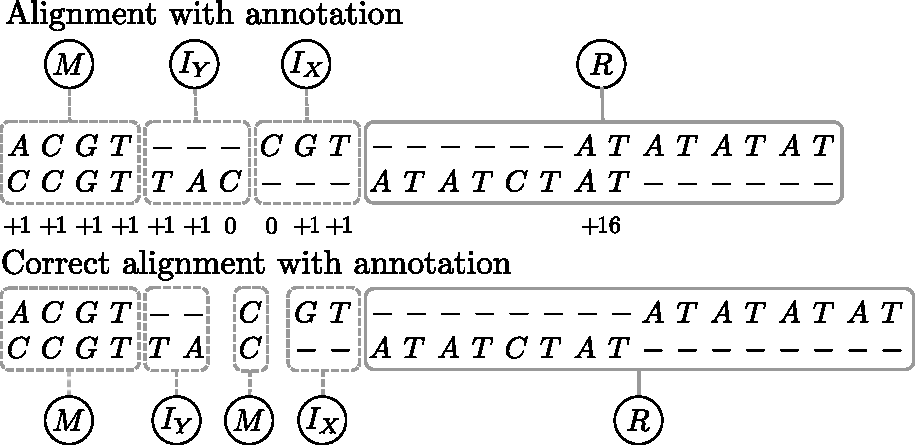
\includegraphics[width=14cm]{../figures/BlockPosterior.pdf}
\end{center}
\caption[Block posterior decoding function]{ 
Explanation of BPD gain function. Gray solid lines represents single
emissions, dashed lines represents multiple emissions (each alignment column is
one emission). Emission from repeat state have gain $+16$ because it emits $16$
sequences in exactly same regions of the input sequences.  Other alignment
columns get $+1$ only if there is same alignment column in the correct
alignment that was generated by same state.

}\label{FIGURE:BLOCK_POSTERIOR} 
\end{figure}

The reason for using $+l$ instead of $+1$ is that otherwise decoding method
would be biased towards short blocks. Instead of $l$, the number of emitted
symbols, we could use the number of emitted columns. However we would then
discriminate the submodels that would tried to align repeats (although we did
not used such model). Example of this gain function in in the Figure
\ref{FIGURE:BLOCK_POSTERIOR}.

To optimize this gain function, we have to compute posterior probabilities for
all emissions. In generalized pHMM, emission is given by two intervals; one in the
sequence $X$ and one in the sequence $Y$. The number of possible emissions is
$O(n^2m^2)$. The expected gain of the emission is the posterior probability
multiplied by the number of emitted symbols. After computing expected gains of
individual blocks we can compute the highest scoring annotated alignment in
$O(n^2m^2)$ time.

Let $E$ be the number of transitions in the repeat submodel. The naive
computation of the expected gain for the pair of intervals of length $n'$ and
$m'$ can be computed in $O(n'm'E)$ time by forward algorithm for generalized
pair HMM, which would lead to $O(n^3m^3E)$ algorithm for computing posterior
probabilities by forward-backward algorithm. By using proper preprocessing that
can be done in $O((n^2+m^2)E)$ time, we can lower the time complexity of
computing expected gain for an pairs of intervals to $O(k)$ where $k$ is the
number of sunflower submodels (in case of TTP, $k=1$).

Let consider the repeat submodel $H$ with $k$ sunflower pairs $S^X_1, S^Y_1,
\dots, S^X_k, S^Y_k$. Let $p_i$ be the probability of entering sunflower
$S^X_i$.  The probability of transition from $S^X_i$ to $S^Y_i$ is $1$. We can
write the probability of generating arbitrary pair of sequences $X'$ and $Y'$ by $H$ as
\begin{equation}
\prob{X', Y'\mid H} = \sum_{i=1}^k p_i\prob{X'\mid S^X_i}\prob{Y'\mid S^Y_i}
\end{equation}
By pre-computing all of the terms $\prob{X'\mid S^X_i}$ and $\prob{Y'\mid
S^Y_i}$, we can compute the posterior probability of the block in $O(k)$ time.
Naive computation of all $\prob{X'\mid S^X_i}$ would take $O(n^3E)$ time, but
this can be further improved. When computing $\prob{X'\mid S^X_i}$ using the
forward algorithm, we can use the values from the forward table to compute the
probability of emitting any prefix of $X'$ by looking at the forward
probability of final state for the corresponding column. We need to run forward
algorithm only for sequences $X[i:]$ for all $0\leq i< n$. The optimization for
the other sequence is analogous. By using these techniques we can pre-compute
the emission terms in $O((n^2+m^2)E)$ time. Therefore the overall time
complexity of the BPD is $O(kn^2m^2 + (n^2+m^2)E)$. By
same techniques we can optimize the BVA with same time
complexity.

\paragraph{Post-processing}
The problem with the SFF and the TTP models is that they model repeat sequences
independently and do not try to align tandem repeats at orthologous locations.
Therefore we postprocess alignment using 3-state pHMM by realigning segments of
alignments that are annotated as repeats. We also include adjacent gaps into
this postprocess step.

\section{Optimizations}\label{SECTION:REPOPT}

In this section we summarize additional techniques we have used to decrease the
running time of the decoding algorithms. The fastest decoding algorithms described
above run in $O(nmE)$ time, which is still prohibitive for longer sequences.
Additionally, block-based methods are even slower. We used following
optimizations:
\begin{itemize}[itemsep=-1mm]
\item We implemented standard technique of banding. We restrict the alignment
to the window around the guide alignment, that can be obtained by faster but less
precise alignment algorithms. We used Muscle \cite{Edgar2004} with default
parameters to compute guide alignment. The final alignment methods were
restricted to be within 30 bases from the guide alignment. This technique
reduce the $O(nm)$ term from the time complexity to $O((n+m)d)$ where $d$ is
the distance from the guided alignment.

\item The size of the SFF model is enormous. It is not practical to use model
with $310,091$ sunflower pairs. Therefore we used the TRF program
\cite{Benson1999} to find the consensus motifs in the input alignment and used
only those to build SFF model. Note that the transition probabilities to
sunflower pairs were kept same as in the original model. In case that TRF did
find consensus that was not in the original set of consensuses, we assign it
the probability of the least occurring consensus from the original set. This
technique was not applicable to TTP model.

\item To further reduce running time of the BVA and BPD, we restrict the
emissions of the state $R$ to specific intervals in both input sequences. At
first, we found the candidate set of tandem repeat intervals for both input
sequences $X$ and $Y$ independently. Let $T_X$ and $T_Y$ are the sets of
candidate intervals (not necessarily disjoint) for sequences $X$ and $Y$
respectively. We restrict emission of $R$ state only to the pairs of intervals
$i_X, i_Y$ where $i_X$ and $i_Y$ have beginning and end within $10$ bases from
some interval from $T_X$ and $T_Y$ respectively, or if one of $i_X$ or $i_Y$ is
an empty interval (there can be a tandem repeat in only one sequence).  By this
heuristic, $R$ state do emissions in at most $(400|T_X|+n)(400|T_Y|+m)$
positions. We applied this method to both SFF and TPP models.

We used following algorithm to select candidate intervals $T_X$ and $T_Y$:
\begin{enumerate}[itemsep=-1mm]
\item Run the TRF program on the input sequences $X$ and $Y$. Obtain sets of
intervals $T_X$ and $T_Y$ and lists of consensuses $C_X$ and $C_Y$.

\item For every consensus $c\in C_X\cup C_Y$, build the SRF model $S_c$
(sunflower repeat finding model from Section \ref{SECTION:SUNFLOWERMODEL}). 

\item Each model $S_c$ is run on the sequences $X$ and $Y$ using the Viterbi
algorithm. All found repeat intervals are added into corresponding sets $T_X$
and $T_Y$.

\end{enumerate}
The reason for using this method instead of using only intervals from TRF is
that running TRF on the input sequences independently can cause several
problems. At first, if sequence $X$ contain three repetition of motif $m$ and
sequence $Y$ contain only one, then TRF would return interval only for the
sequence $X$. Additionally, consensus can be found in both sequences but can be
rotated, and therefore intervals in both sequences would be shifted.

\end{itemize}

\section{Experiments}

This section summarizes the details of the simulation experiment and measures
we were using for evaluation. At first, we estimated parameters of the model
using annotated human-dog alignment by TRF program \cite{Benson1999}.
Parameters for 3-state model, and 3-state submodel of SFF and transitions to
the repeat state were therefore trained by supervised learning. Setting SFF and
TTP parameters was discussed in the sections \ref{SECTION:SUNFLOWERMODEL} and
\ref{SECTION:TANTAN}.

We sampled 200 test alignments each of length at least 200 bases from the SFF
submodel with the condition, that the number of repetitions in the tandem
repeat has to be at least three in both sequences. Reason for this is that
otherwise we would have segments of alignments that are annotated as repeats,
but in fact are not because it would contain only one copy of the motif. We
refer to these alignments (along with sampled repeat annotation) as the correct
alignments and correct annotation (repeat intervals and consensuses).  The
program Context \cite{Hickey2011} was trained of the 200 separate alignments
sampled from the model. 


We used the same model for evaluation of parameters. To evaluate the robustness
of our method, we assess the effects of misspecification of the parameters by
estimating model parameters from human-chicken alignment and perturbing model
parameters (details are in the next section).

\paragraph{Measures:} The first measure we used was the error rate: the
fraction of incorrectly predicted columns of an alignment. It was measured only
on the alignment columns generated from non-repeats states during sampling.
Reason for this is that SFF and TTP does not model alignment of repetitive
regions.

Additionally, we investigate the precision of predicting exact repeat block
boundaries in alignments by measuring the number of correctly predicted repeat
blocks; block is correctly predicted if it contain identical parts of sequences
as the corresponding block in the correct alignment. We report the block
sensitivity, which is the fraction of the number of correctly predicted blocks
and the number of correct block, and block specificity, which is the fraction
of the number of correctly predicted blocks and all predicted blocks. We also
investigate the accuracy of prediction of repeat annotation for individual
alignment columns; the repeat sensitivity and specificity.

We also measured the relation of the error rate and the distance
from the nearest repeat. Alignment column was considered as repeat if in the
correct alignment at least one base of the column was annotated as an repeat.
The distance is measured by the number of columns. This measure is important,
because when the distance from the repeat is high, our model is identical to
3-state pHMM and therefore the performance of both models should be similar in
such regions. However, we do expect models incorporating repeats to be more
precise in the regions near tandem repeats.

\section{Results of the Simulation Experiments}\label{SECTION:REPSIMRESULTS}

This section discuss the results of the simulation experiment. We split results
of various version of algorithms into several tables. The results for SFF and
TTP models are in the Table \ref{TABLE:SFFMAIN}. Table
\ref{TABLE:SFFMAINORIGINAL} contain results for same algorithms, but with use
of the correct intervals and motifs instead of of their approximations obtained
by TRF program. Results for the non-SFF alignment programs and methods for
aligning sequences with repeats is in the Table \ref{TABLE:SFFOTHER}. The
effects of misspecification of mode parameters is in the Table
\ref{TABLE:SFFMARGINALIZED} and the effects of different masking methods on
posterior and Viterbi algorithm is in the table \ref{TABLE:SFF3STATEMASK}.
Figure \ref{FIGURE:SFF_GRAPHS} compare the relation between the error rate and
the distance from the repeat for studied methods. Following text contain the
discussion of the results.

\def\M{$^\circ$} % mark by a star
\def\MM{$^{\circ\circ\circ}$} % mark by two stars
\def\D{$^{\circ\circ}$} % mark by dagger
\def\DD{$^{\dagger}$} % mark by dagger
\def\R{$^{\yen}$}
\def\RR{$^{\yen\yen}$}
\def\CC#1{\multicolumn{1}{c}{#1}} % center column
\def\S{$^{\star}$}

\begin{table*}
\begin{center}
\begin{tabular}{lr@{\quad}rr@{\quad}rr}
\hline
          & \CC{Alignment} & \multicolumn{2}{c}{Repeat} & 
\multicolumn{2}{c}{Block}\\
Algorithm & \CC{error} & \CC{sn.} & \CC{sp.} & \CC{sn.} & \CC{sp.} \\
\hline
\hline
%\hline
3-state VA (baseline)    & 4.78\% \\
\hline
SFF MPD   & {\bf 3.37\%} & {\bf 95.97\%} & 97.78\% & {\bf 43.07\%} & 44.87\%\\
SFF PD    & 3.53\% & 95.86\% & 97.87\% & 42.70\% & 47.37\%\\
SFF BPD   & 3.51\% & 93.09\% & {\bf 98.07}\% & 36.50\% & 41.67\%\\
SFF BVA   & 3.91\% & 93.26\% & 97.96\% & 35.77\% & 40.66\%\\
SFF VA    & 4.04\% & 95.29\% & 97.85\% & 42.70\% & {\bf 48.95\%}\\
TANTAN BPD& 5.05\% & 61.38\% & 97.48\% & 0.00\% & 0.00\%\\
TANTAN BVA& 6.17\% & 67.86\% & 96.51\% & 0.00\% & 0.00\%\\
\hline
\end{tabular}
\end{center}
\caption{Accuracy of decoding methods on simulated data.}\label{TABLE:SFFMAIN}
\end{table*}

Since we run the decoding algorithms described in the section
\ref{SECTION:REPDECODING} with various combination of additional information
(i.e. repeat intervals and motifs), we use following symbols to
distinguish them.

\begin{itemize}[itemsep=-1mm]

\item[\M] method uses the correct motifs. 

\item[\D] method uses intervals from the correct repeat blocks.

\item[\MM] method uses the correct motifs and intervals from the
correct repeat blocks.

\item[\R] Parameters of the three-state submodel were estimated from
human-chicken alignment. 

\item[\RR] Parameters of SFF submodel were perturbed randomly.

\item[\DD] Columns with at least one masked character are considered as
repeats.

\item[\S] Non-overlapping set of repeats from TRF output with maximal total
score is used.

\end{itemize}

In general, using SFF model decreased the alignment error rate by $15-30\%$ as
opposed to baseline method as can be seen in table \ref{TABLE:SFFMAIN}. The
$15\%$ decrease was obtained by replacing 3-state model with the Sunflower Field
model, other improvements were through using different decoding algorithms,
with the marginalized posterior decoding having the lowest error rate. The
Viterbi based methods had consistently higher error rate than posterior based
methods and the block-based versions of the algorithms decreased the error rate
by at most $3.3\%$ as opposed to non-block based methods. Surprisingly, block
based methods had poorest performance in the block sensitivity and specificity
and repeat sensitivity. These measures are closer to what block methods
optimize, so we expected opposite. Reason for this is perhaps due to
approximate {intervals and/or motifs obtained TRF and SRF}, since when running
algorithms that uses correct intervals and motifs (see Table
\ref{TABLE:SFFMAINORIGINAL}), their performance improved significantly.
Results in Table \ref{TABLE:SFFMAINORIGINAL} helps us to quantify the effect of
not using the exact repeat intervals and also can be used as an upper bounds
for the performance of our models. There is clearly room for improvements of
repeat intervals, we could perhaps try to use other programs that detect tandem
repeats, like ATRhunter \cite{Wexler2005} or mreps \cite{Kolpakov2003}.

\begin{table*}
\begin{center}
\begin{tabular}{lr@{\quad}rr@{\quad}rr}
\hline
          & \CC{Alignment} & \multicolumn{2}{c}{Repeat} & 
\multicolumn{2}{c}{Block}\\
Algorithm & \CC{error} & \CC{sn.} & \CC{sp.} & \CC{sn.} & \CC{sp.} \\
\hline
\hline
%\hline
3-state VA (baseline)    & 4.78\% \\
\hline
SFF MPD\M            & {\bf 3.02}\% & {\bf 98.93}\% & 99.64\% & 77.01\% & 76.17\% \\ 
SFF PD\M             & 3.42\% & 98.84\% & 99.51\% & 75.91\% & 80.93\% \\
SFF BPD\MM           & 3.21\% & 97.70\% & 99.87\% & 80.66\% & {\bf 94.44}\% \\
SFF BVA\MM           & 3.71\% & 98.12\% & 99.85\% & {\bf 81.75}\% & 92.18\% \\
SFF VA\M             & 3.94\% & 98.54\% & 99.45\% & 75.55\% & 83.47\% \\
TANTAN BPD\D         & 3.42\% & 60.45\% & {\bf 99.90}\% & 0.36\% & 0.46\% \\
TANTAN BVA\D         & 3.83\% & 61.74\% & 99.88\% & 0.00\% & 0.00\% \\
\hline
\end{tabular}
\end{center}
\caption{Accuracy of decoding methods using real motif and/or real intervals on simulated data.}\label{TABLE:SFFMAINORIGINAL}
\end{table*}

Similar behaviour was obtained for TTP model; using the original intervals, TTP
model has only slightly worse error rate than the SFF, which is expectable, since
the data were generated from the SFF model. However, using TRF for intervals,
TTP has significantly higher error rate, which means that TTP is even more
sensitive to the intervals that are used. Also the high error rate and low
repeat and block prediction performance could be caused by improperly treating
the first repetition, because annotations of TTP methods almost always skip the
first copy of repeat motif. Additionally, in TPP the motifs in tandem repeat
are not dependent between sequences, which can be also source of higher error
rate.  This could be improved by merging the chain of prefix states $P_1,
\dots, P_K$ into chain of match states aligning the first repetition.

Results of other alignment methods are in the Table \ref{TABLE:SFFOTHER}.
Namely the Context program, Muscle, 3-state posterior algorithm and 3-state
posterior algorithm with hard-masking. Apart from the 3-state posterior
algorithm, all methods had higher error rate than the baseline method. The high
error rate of the Context program could be caused by insufficient training data
or some software issues. We run muscle with default parameters and therefore
its scoring scheme was not tailored to our method. Using the hard-masking
produced alignment with higher error rate. It might be cause by the
insufficient accuracy of the tandem repeat annotation.

\begin{table*}
\begin{center}
\begin{tabular}{lr@{\quad}rr@{\quad}rr}
\hline
          & \CC{Alignment} & \multicolumn{2}{c}{Repeat} & 
\multicolumn{2}{c}{Block}\\
Algorithm & \CC{error} & \CC{sn.} & \CC{sp.} & \CC{sn.} & \CC{sp.} \\
\hline
\hline
%\hline
3-state VA (baseline)    & {4.78}\% \\
\hline
Context             & 5.98\% \\
Muscle              & 5.62\% \\
3-state PD   & \bf 4.41\% \\
3-state masked PD\DD & 5.03\% & 99.23\% & 74.16\% & 7.66\% & 7.24\%\\
\hline
\end{tabular}
\end{center}
\caption{Accuracy for standard algorithms and other tools on the simulated data.
Most of the methods did not annotate the alignment with tandem repeats and
therefore relating metrics are not available.
}\label{TABLE:SFFOTHER}
\end{table*}

Since we did use the same model for generating data and testing, we tried to
quantify the effect of misspecification of the model parameters.  SFF model
have two principal types of parameters; parameters of the 3-state HMM and
parameters of the Sunflower model. We investigate the effect of
{misspecification} for both types independently. For the parameters of 3-state
model, we have estimate the parameters from human-chicken alignments instead of
human-dog alignment. For the second type, we have perturbed the each parameter
of Sunflower model randomly by additive term from $0.02$ to $0.05$. On these
models we run marginalized posterior decoding. Table
\ref{TABLE:SFFMARGINALIZED} shows that our method is quite robust. Our method
is more sensitive to change in the training alignment, since the error rate for
MPD increased by $8\%$, but it is still significantly better than the baseline
method. Perturbing parameters for Sunflower submodel did not have significant
effect on error rate (increase by $0.5\%$). 

\begin{table*}
\begin{center}
\begin{tabular}{lr@{\quad}rr@{\quad}rr}
\hline
          & \CC{Alignment} & \multicolumn{2}{c}{Repeat} & 
\multicolumn{2}{c}{Block}\\
Algorithm & \CC{error} & \CC{sn.} & \CC{sp.} & \CC{sn.} & \CC{sp.} \\
\hline
\hline
%\hline
3-state VA (baseline)    & 4.78\% \\
\hline
SFF MPD    & 3.37\% & 95.97\% & 97.78\% & {\bf 43.07\%} & {\bf 44.87}\%\\
SFF MPD\R & 3.63\% & {\bf 96.03\%} & 97.74\% &  42.70\% &  43.33\% \\ 
SFF MPD\RR & {\bf 3.36}\% & 95.99\% & {\bf 97.81}\% & 40.88\% & 43.08\% \\ 
SFF MPD\M  & \bf 3.02\% & \bf 98.93\% & \bf 99.64\% &\bf 77.01\% &\bf 76.17\% \\ 
\hline
\end{tabular}
\end{center}
\caption{Accuracy for marginalized posterior decoding with different models or real motifs.
The best and the second best are bold.} \label{TABLE:SFFMARGINALIZED}
\end{table*}

Table \ref{TABLE:SFF3STATEMASK} investigates the use of the different repeat
finding methods for masking. We used the Sunflower model (modified for finding
tandem repeats as described in section \ref{SECTION:SUNFLOWERMODEL}), TRF, and
TRF with non-overlapping repeats (we select maximal scoring non-overlapping set
of tandem repeats out of TRF output). We used hard-masking as described in
section \ref{SECTION:REPALNMETHODS}. For decoding we used both the VA and the
PD.  Apart from  using correct intervals, the best performing masking was used
with non-overlapping repeats from TRF.

\begin{table*}
\begin{center}
\begin{tabular}{lr@{\quad}rr@{\quad}rr}
\hline
          & \CC{Alignment} & \multicolumn{2}{c}{Repeat} & 
\multicolumn{2}{c}{Block}\\
Algorithm & \CC{error} & \CC{sn.} & \CC{sp.} & \CC{sn.} & \CC{sp.} \\
\hline
\hline
%\hline
3-state Viterbi (baseline)    & 4.78\% \\
\hline
3 state masked PD, TRF\DD       &5.03&{\bf 99.23}&74.16&7.66&7.24\\
3 state masked PD, Sunflower\DD &5.21&98.30&68.65&{\bf 9.12}&7.53\\
3 state masked PD, TRF\S\DD     &{\bf 4.77}&88.17&{\bf 79.63}&7.66&{\bf 9.13}\\
3 state masked PD, \MM\DD       &{\bf 4.50}&{\bf 100.00}&{\bf 97.23}&{\bf 45.99}&{\bf 61.13}\\
\hline
3 state masked VA, TRF\DD         &5.89&{\bf 99.25}&73.29&5.47&5.14\\
3 state masked VA, Sunflower\DD   &5.82&98.32&67.90&{\bf 5.84}&4.89\\
3 state masked VA, TRF\S\DD       &{\bf 5.10}&88.33&{\bf 78.68}&5.47&{\bf 6.47}\\
3 state masked VA, \MM\DD         &{\bf 5.02}&{\bf 100.00}&{\bf 95.41}&{\bf 45.99}&{\bf 44.21}\\
\hline
\end{tabular}
\end{center}
\caption{Accuracy of decoding method using simple 3-state HMM and hard-masking. The best and the second best are bold. }\label{TABLE:SFF3STATEMASK}
\end{table*}

Finally, we investigate the relation between the error rate and the distance
from the nearest repeat. Figure \ref{FIGURE:SFF_GRAPHS} contains graphs for
this metric for various combination of parameters. In general, all algorithms
have highest error rate near boundaries of the repeat, with the error rate lowering
with the distance from the repeat. Most methods reach the baseline error rate
within distance $10$ bases of the repeat border.

\begin{figure}
\begin{center}
\begin{subfigure}{0.5\textwidth}
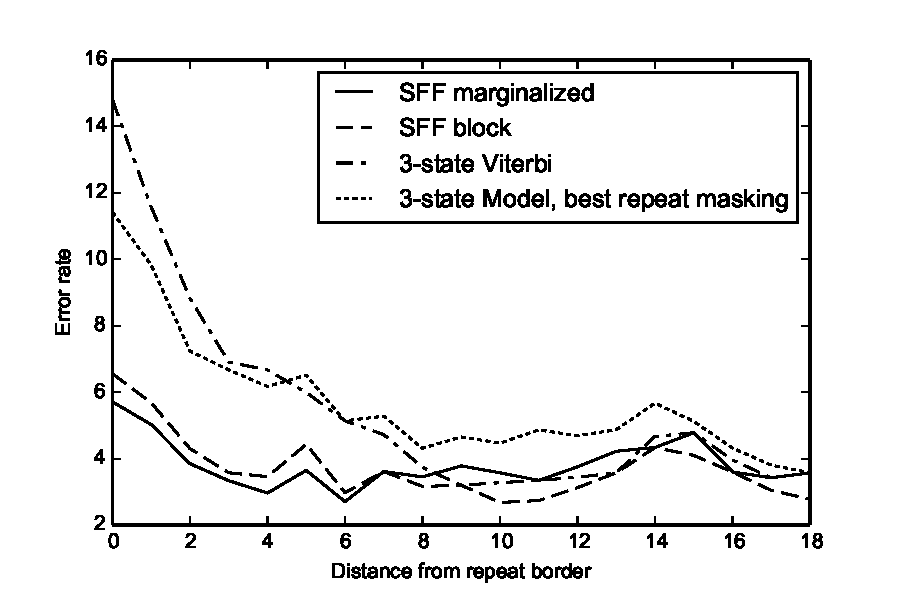
\includegraphics[width=\textwidth]{../figures/error_graph_overview.pdf}
\caption{Our methods and traditional methods}\label{FIGURE:SFFOVER}
\end{subfigure}%
\begin{subfigure}{0.5\textwidth}
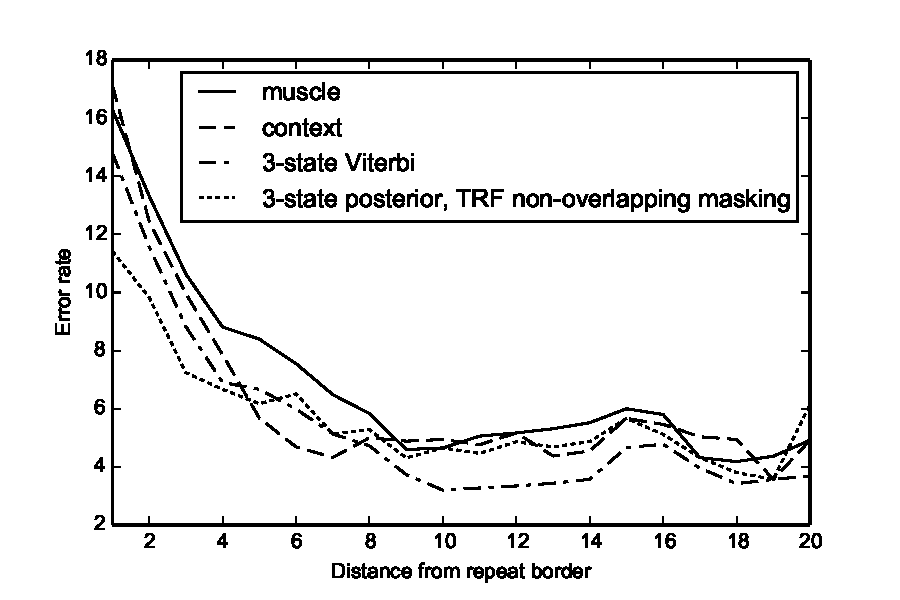
\includegraphics[width=\textwidth]{../figures/error_graph_other.pdf}
\caption{Other methods}\label{FIGURE:SFFOTHER}
\end{subfigure}%

\begin{subfigure}{0.5\textwidth}
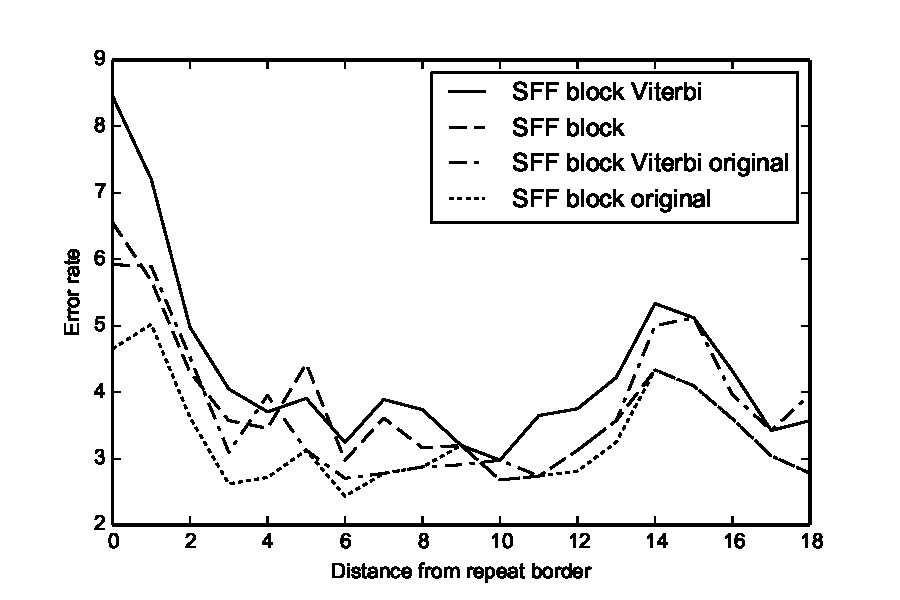
\includegraphics[width=\textwidth]{../figures/error_graph_sffblock.pdf}
\caption{Block decodings}\label{FIGURE:SFFBLOCKS}
\end{subfigure}%
\begin{subfigure}{0.5\textwidth}
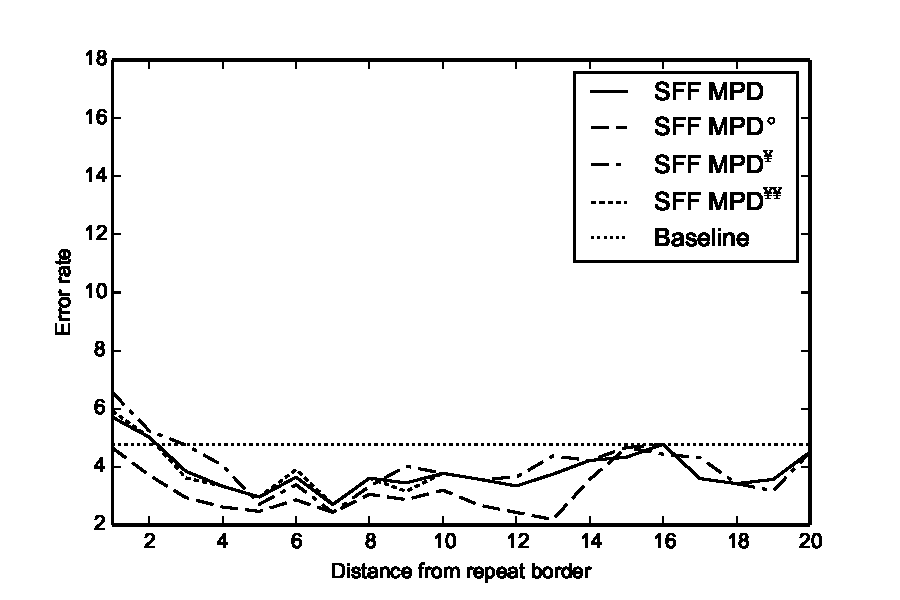
\includegraphics[width=\textwidth]{../figures/error_graph_marginalized.pdf}
\caption{Same method, different models}\label{FIGURE:SFFWEIRD}
\end{subfigure}%

\begin{subfigure}{0.5\textwidth}
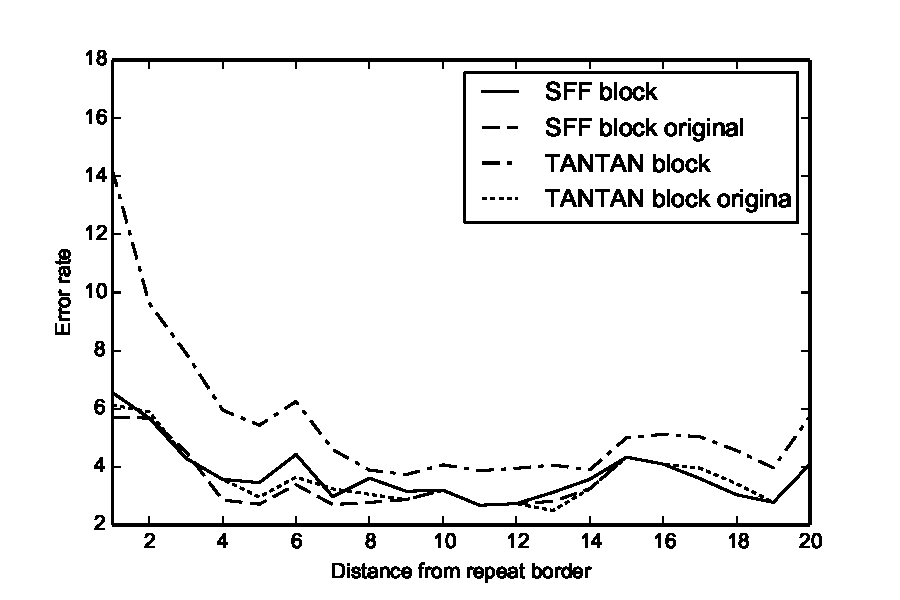
\includegraphics[width=\textwidth]{../figures/error_graph_sffvstantan.pdf}
\caption{Sunflower and TANTAN}\label{FIGURE:SFFTANTAN}
\end{subfigure}%
\begin{subfigure}{0.5\textwidth}
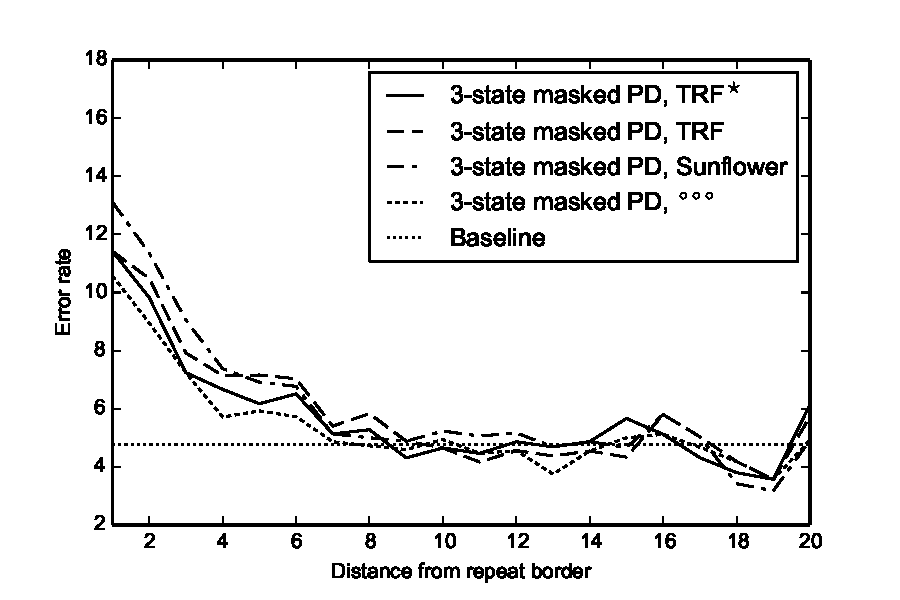
\includegraphics[width=\textwidth]{../figures/error_graph_3statemasking.pdf}
\caption{Different methods of masking}
\end{subfigure}%
\caption{
The relation between the error rate and the distance from the nearest repeat. On the Y
axis is error rate of the algorithm; the number of incorrectly aligned columns.
On the X axis is the distance from the nearest repeat. Baseline is the overall
error rate, with no relation to the distance from the repeat border, for
3-state model with the VA.
}\label{FIGURE:SFF_GRAPHS} 
\end{center}
\end{figure}

Figures \ref{FIGURE:SFFOVER} and \ref{FIGURE:SFFOTHER} suggests that the right
selection of decoding method can improve error rate near repeats, but most of
the drop in the error rate was caused by using SFF model. As with other
metrics, TTP with correct intervals performs similarly to SFF model, but TTPs
error rate near repeats raises significantly where intervals were obtained from
TRF (see Figure \ref{FIGURE:SFFTANTAN}). Using different  model did not have
large effect also on the error rate as we can see in the Figure
\ref{FIGURE:SFFWEIRD}. Figure \ref{FIGURE:SFFBLOCKS} demonstrates that for
block methods, using block Viterbi double the error rate near repeat.


\begin{comment}
\section{Possible Improvements}

\begin{reformulate*}
Sem by som mohol napisat, ako by sa dal pouzit symetricky model s cyklom
stavov, alebo ako by sa dal ten cyklus stavov odstranit odstranenim jednej
hrany a pridanych n hran -- co je lepsie ako pridat n vrcholov.
\end{reformulate*}
\end{comment}
\label{LastPage}
